\section{Data Preparation}

Before the classification can be done, a few preparation steps are still
required, namely the assignment of class labels to each instance as
well as feature selection to reduce the set of attributes to an
acceptable size.

\subsection{Assignment of Class Labels}
\label{sec:assignment}

To obtain the class labels used for classification, the
continuous attribute "total number of violent crimes per 100K
population" is divided into separate groups. Each of this groups is
assigned an ordinal class label that can be predicted during classification.
If for example the number of groups is equal to three, one could
assign the labels "High", "Medium" and "Low" to the corresponding
groups.

The simple k-Means clustering algorithm is used to achieve this
by comparing different amounts of groups, i.e. testing
different values of k. Those different k values were compared by using
the elbow-method and \(k=3\) was revealed as the best parameter as
shown in \fref{fig:sse}.
\begin{figure}[H]
  \centering
  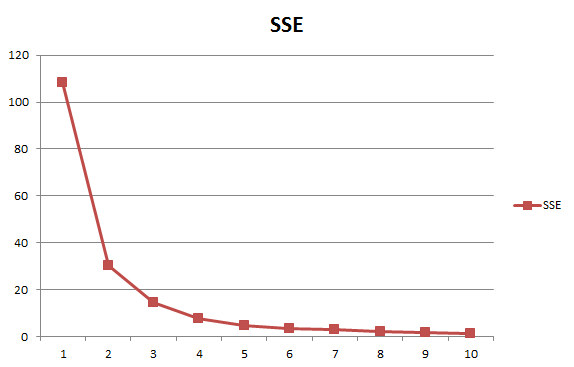
\includegraphics[width=\columnwidth]{../../charts/SSE.png}
  \caption{Sum of the squared errors for different choices of k}
  \label{fig:sse}
\end{figure}
\noindent The three classes originating from this choice are namely
"High", "Medium" and "Low", the percentage boundaries are
respectively:
\begin{description}
  \setlength{\itemsep}{-2pt}
\item[Low:] \([0\%; 22\%]\) 
\item[Medium:] \((22\%; 56\%]\)
\item[High:] \((56\%; 100\%]\)
\end{description}
%% It should be noted, that the authors of \textit{"An Experimental Study
%% of Classification Algorithms for Crime Prediction"} \cite{indian}
%% obtained different results for the percentage boundaries, they did
%% however not disclose the details of their approach.
%% Their percentage boundaries are "Low": \([0\%;25\%)\), "Medium": \([25\%; 40\%)\) and "High": \([40\%; 100\%]\).

\subsection{Feature Selection}
\label{sec:feature_selection}    

To reduce the total of 128 attributes in the dataset to an acceptable
amount, we employed a two-step approach that is presented in the
following sections.

\paragraph{Selection by Judgement of Significance}
First we discussed each attribute separately and agreed whether we
would include it based on its significance. In the course of this
procedure, we obtained a ranking of the attributes we regarded as most
significant.

\paragraph{Comparison with Correlation Ranking}
In the second step, we compared our choices with the attributes that
have the highest correlation with the classes. We found that the
majority of the attributes that we selected based on common sense was
already present in the ranking, however a few attributes like
"population" were discarded because of a correlation near zero.

